\documentclass[a4paper, 11pt]{article}
\usepackage{comment} % enables the use of multi-line comments (\ifx \fi) 
\usepackage{lipsum} %This package just generates Lorem Ipsum filler text. 
\usepackage{fullpage} % changes the margin
\usepackage{amsmath, amssymb,graphicx, subcaption}
\usepackage{algorithm}
\usepackage[noend]{algpseudocode}
\DeclareMathOperator*{\argmax}{arg\,max}
\DeclareMathOperator*{\argmin}{arg\,min}

\begin{document}
%Header-Make sure you update this information!!!!
\section*{Problem-Statement}
Let an object have a reflectance given by $r$. Then the complex-distribution of the object-field is given by $g\sim CN(0,D(r))$ \cite{CaseyOpticallyCoherent}. The problem statement is given 
\begin{eqnarray*}
y=Ag+w
\end{eqnarray*}
we would like to estimate $r$.
\section{Case I: Linear measurements $(A=I)$}
\subsection{Forward-model: }
Let the reflectance of the object that is imaged be given by $r\in[0,1]$. Under the assumed model of the object-filed given by $g\sim CN(0,D(r))$, and the additive white-gaussian noise model we have that the measured complex-signal is given as 
\begin{eqnarray*}
y=g+w.
\end{eqnarray*}
A single-realization of this is given in Figure~\label{fig:forwardModel} with std. deviations of the noise at $\sigma_w=\{0.001,0.1\}$. 
\begin{figure}[h]
\centering
\centering
    \begin{subfigure}[b]{0.22\textwidth}
        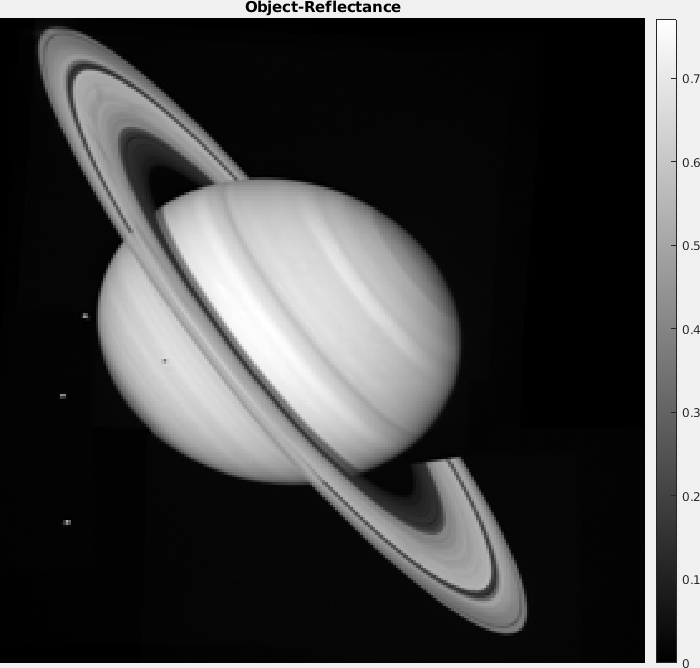
\includegraphics[width=\textwidth]{../Figures/OpticalReflectance.png}
        \caption{Reflectance ($r$)}
        \label{fig:reflectanceObject}
    \end{subfigure}
    \begin{subfigure}[b]{0.22\textwidth}
        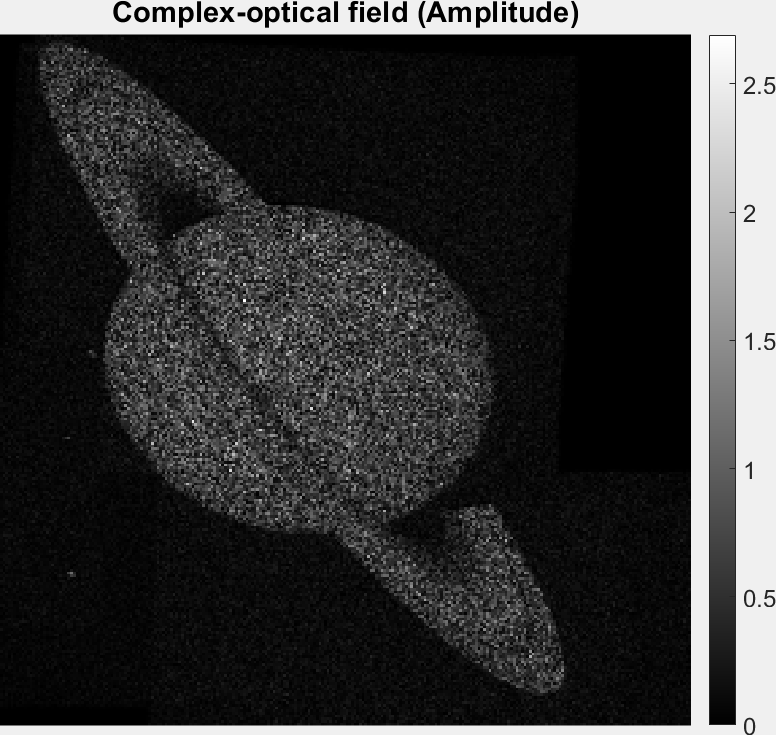
\includegraphics[width=\textwidth]{../Figures/ComplexOpticalFieldAmplitude.png}
        \caption{Optical-Field ($|g|$)}
        \label{fig:opticalField}
    \end{subfigure}
    \begin{subfigure}[b]{0.22\textwidth}
        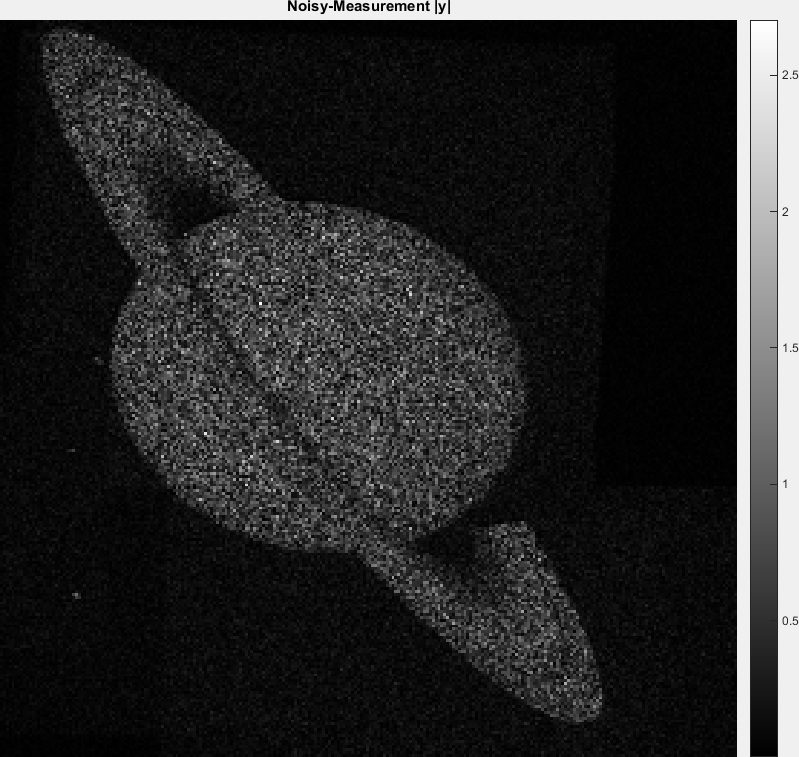
\includegraphics[width=\textwidth]{../Figures/NoisyMeasurementAmplitudeNoiseSigma1e-3.png}
        \caption{($|y|$) $\sigma=0.001$}
        \label{fig:noisyMeasurement1e-2}
    \end{subfigure}
    \begin{subfigure}[b]{0.22\textwidth}
        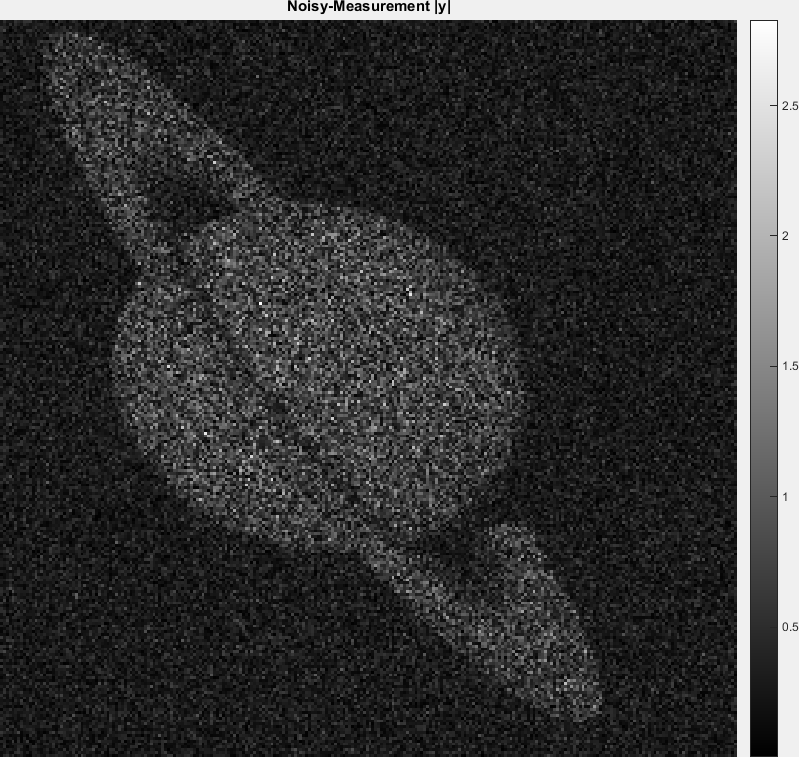
\includegraphics[width=\textwidth]{../Figures/NoisyMeasurementAmplitudeNoiseSigma1e-1.png}
        \caption{($|y|$) $\sigma=0.1$}
        \label{fig:noisyMeasurement1e-1}
    \end{subfigure}
\caption{An example-realization of the forward-model $y=g+w$ . Two realizations of the noisy observations are shown at std. deviations of $\{0.001, 0.1\}$.}
\label{fig:forwardModel}
\end{figure}

\subsection{ML-estimate}
The likelihood of the measurements $y$ is given as $p(y|r)\sim CN(0,D(r)+\sigma_w^2I)$. Applying the maximum-likelihood estimator to the above problem we have  
\begin{eqnarray*}
\hat{r}&=& \argmax \log p(y|r) \\
&=& \argmax \frac{-1}{2} \Bigg( \log\left( (2\pi)^N|D(r)+\sigma_w^2I|\right)+y^H (D(r)+\sigma_w^2I)^{-1}y\Bigg) \\
&=& \argmax \frac{-1}{2} \Bigg( \sum_{i=1}^N \log \left( 2\pi (r_i +\sigma_w ^2)\right) +\frac{|y_i|^2}{r_i +\sigma_w^2}\Bigg) \\
\implies \hat{r_i}&=& \argmax \frac{-1}{2} \Bigg( \log \left( 2\pi (r_i +\sigma_w ^2)\right) +\frac{|y_i|^2}{r_i +\sigma_w^2} \Bigg) \\
&=& \argmin \log \left( 2\pi (r_i +\sigma_w ^2)\right) +\frac{|y_i|^2}{r_i +\sigma_w^2}.
\end{eqnarray*}
Taking the differential of the above equation and equating to zero we get the ML estimate   
\begin{eqnarray*}
\hat{r}_i&=&|y_i|^2-\sigma_w^2.
\end{eqnarray*}
The reconstructions for varying degrees of noise is shown in Figure~\ref{fig:inversionModel} (a-d). 
\begin{figure}[h]
\centering
\centering
    \begin{subfigure}[b]{0.22\textwidth}
        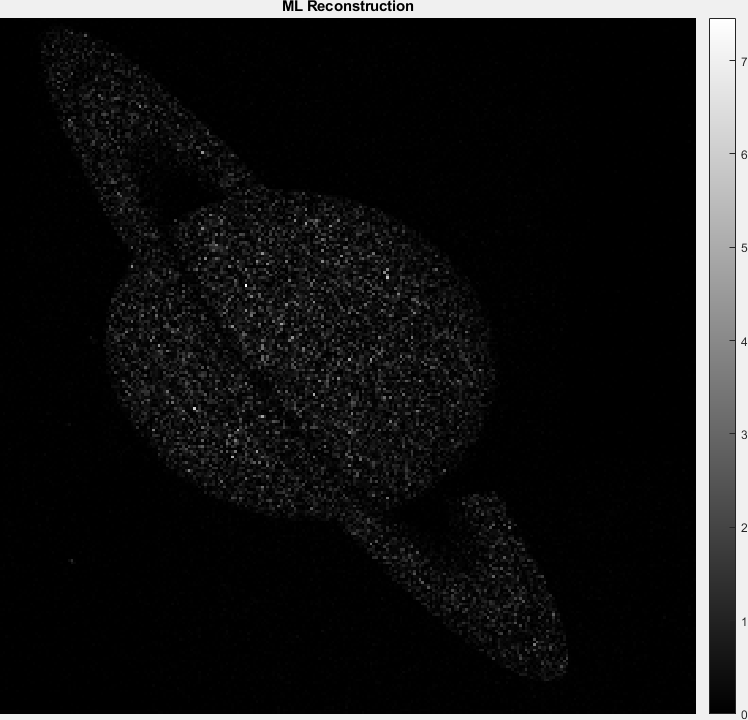
\includegraphics[width=\textwidth]{../Figures/MLReconstructionNoiseSigma1e-2.png}
        \caption{ML ($\sigma=1e^{-2}$)}
        \label{fig:ML-2}
    \end{subfigure}
    \begin{subfigure}[b]{0.22\textwidth}
        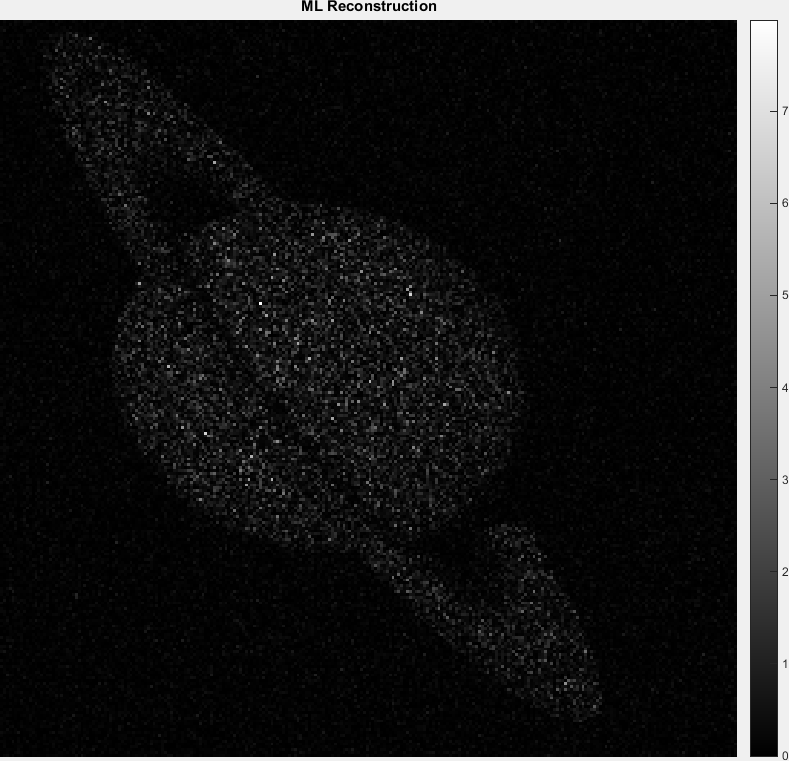
\includegraphics[width=\textwidth]{../Figures/MLReconstructionNoiseSigma1e-1.png}
        \caption{ML ($\sigma=1e^{-1}$)}
        \label{fig:ML-1}
    \end{subfigure}
    \begin{subfigure}[b]{0.22\textwidth}
        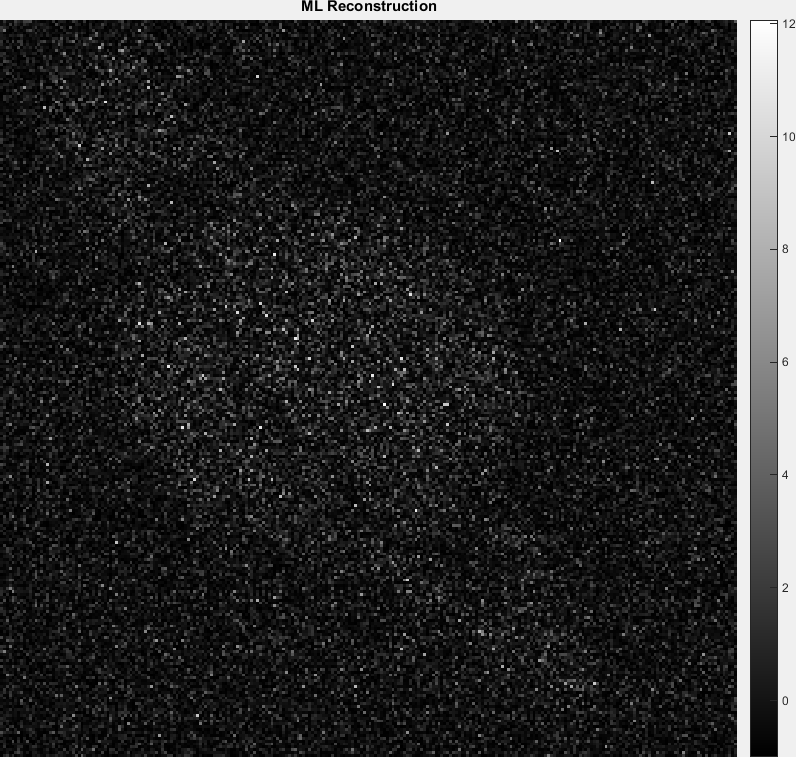
\includegraphics[width=\textwidth]{../Figures/MLReconstructionNoiseSigma1e0.png}
        \caption{ML ($\sigma=1e^{0}$)}
        \label{fig:ML0}
    \end{subfigure}
    \begin{subfigure}[b]{0.22\textwidth}
        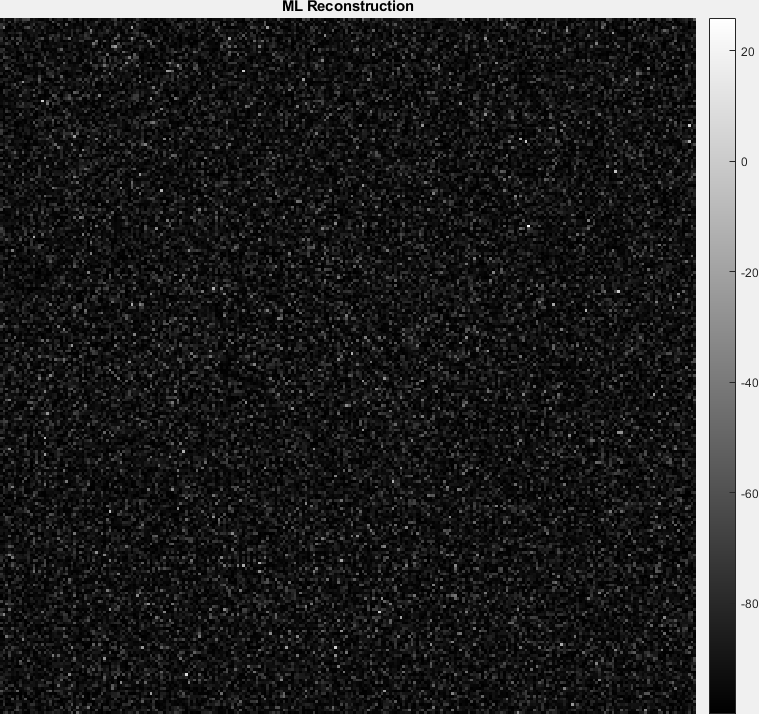
\includegraphics[width=\textwidth]{../Figures/MLReconstructionNoiseSigma1e1.png}
        \caption{ML ($\sigma=1e^{1}$)}
        \label{fig:ML1}
    \end{subfigure}
    \begin{subfigure}[b]{0.22\textwidth}
        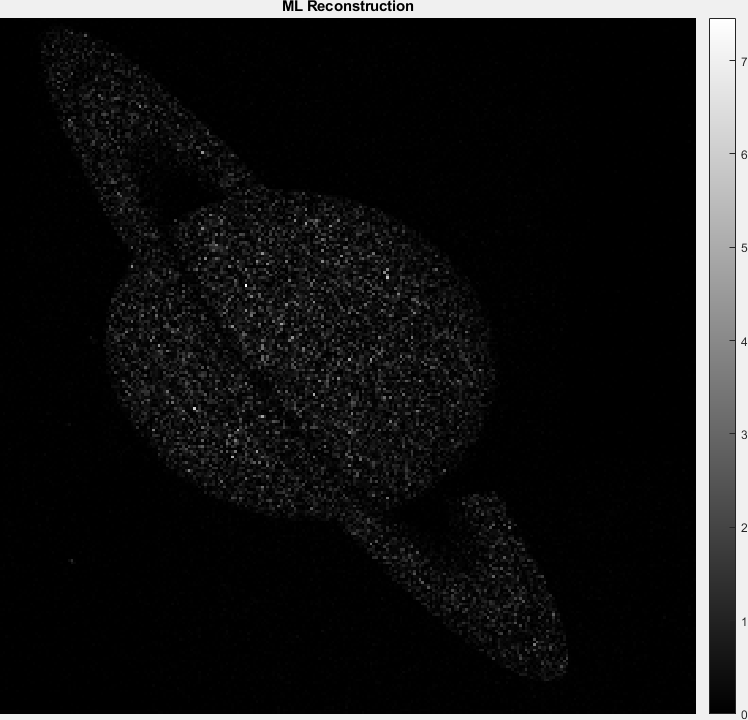
\includegraphics[width=\textwidth]{../Figures/MLReconstructionNoiseSigma1e-2.png}
        \caption{PnP ($\sigma=1e^{-2}$)}
        \label{fig:PnP-2}
    \end{subfigure}
    \begin{subfigure}[b]{0.22\textwidth}
        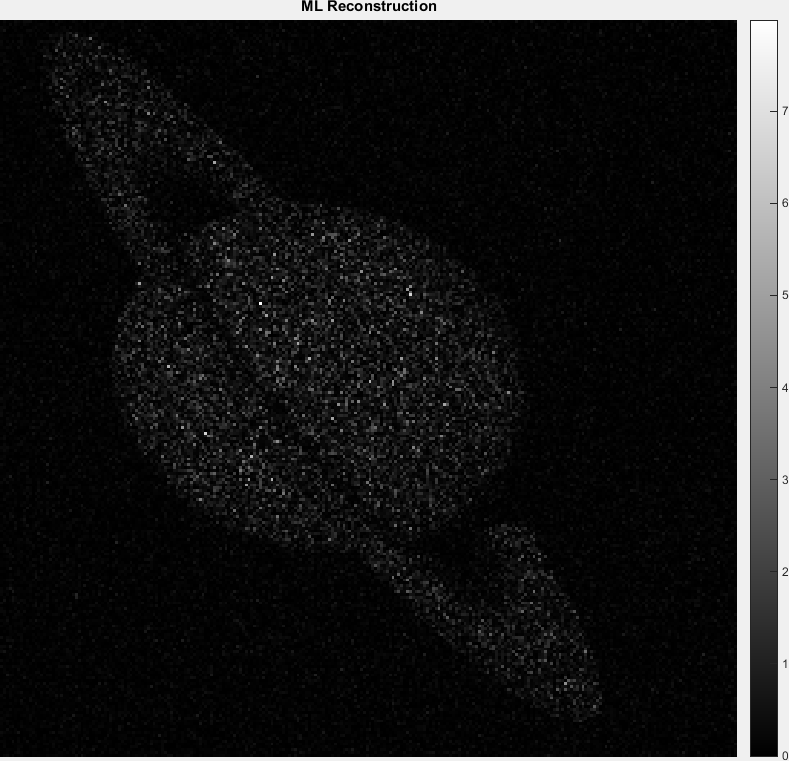
\includegraphics[width=\textwidth]{../Figures/MLReconstructionNoiseSigma1e-1.png}
        \caption{PnP ($\sigma=1e^{-1}$)}
        \label{fig:PnP-1}
    \end{subfigure}
    \begin{subfigure}[b]{0.22\textwidth}
        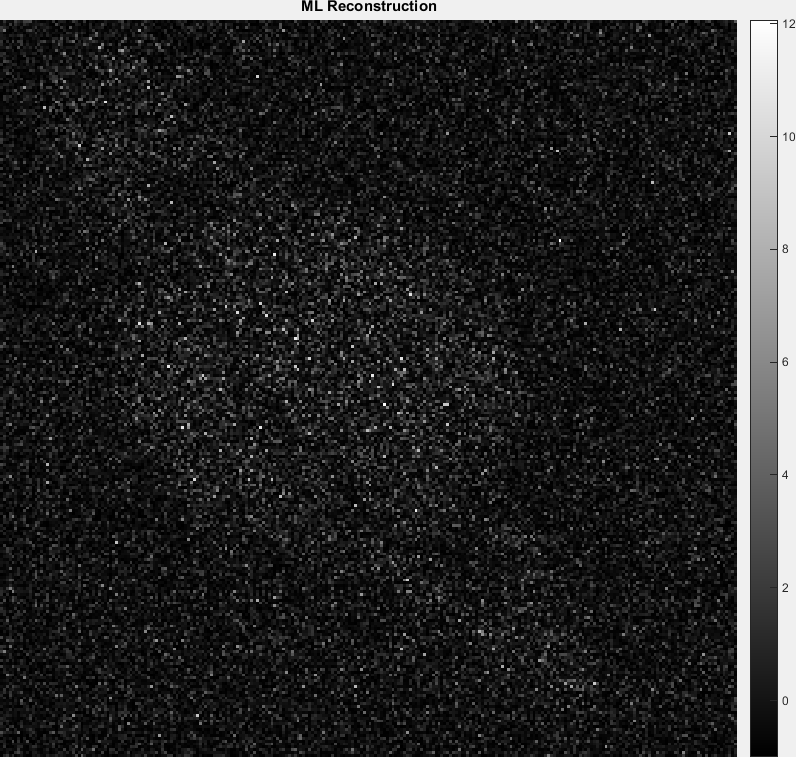
\includegraphics[width=\textwidth]{../Figures/MLReconstructionNoiseSigma1e0.png}
        \caption{PnP ($\sigma=1e^{0}$)}
        \label{fig:PnP0}
    \end{subfigure}
    \begin{subfigure}[b]{0.22\textwidth}
        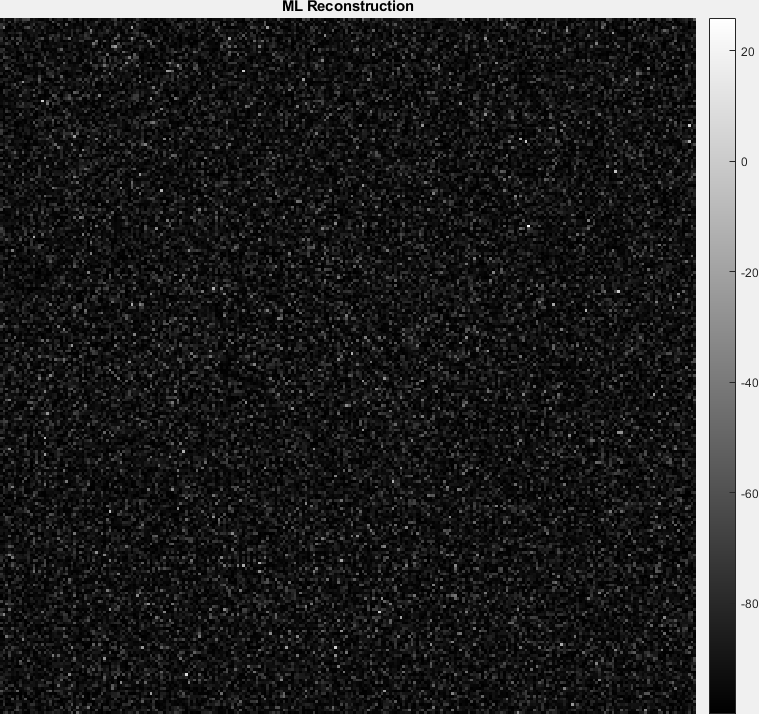
\includegraphics[width=\textwidth]{../Figures/MLReconstructionNoiseSigma1e1.png}
        \caption{PnP ($\sigma=1e^{1}$)}
        \label{fig:PnP1}
    \end{subfigure}
\caption{An example-realization for different inversion-models. The inversions are shown for different std. deviations of $\{0.01,0.1, 1,10\}$.}
\label{fig:inversionModel}
\end{figure}
\subsection{Plug and play (PnP) estimate (MAP)}
The MAP estiamate for the above problem is given as 
\begin{eqnarray}
\hat{r}&=& \argmin -\log p(r|y) \notag\\
&=& \argmin  -\log p(y|r)-\log p(r). \label{eq:MAPestimate}
\end{eqnarray}
The PnP algorithm \cite{PnPalgorithm} decouples the above problem into one where we can apply the forward and prior models in the form of denoisers. Specifically, the PnP algorithm operates by splitting the unknown variable $r$ into two variables $r,v$ and converts the unconstrained optimization problem in (\ref{eq:MAPestimate}) into a constrained optimization problem 
\begin{eqnarray} 
\hat{r}=\underset{r=v}{\argmin} \,\, \ell (r)+\beta s(v)
\end{eqnarray}
where $\beta s(v)=p(v)$ is the prior term and $\ell (r)$ enforces the meausrement constraints on $r$. Adopting an ADMM approach to solve the above problem results in an algorithm containing two primary operations:\\ \\(1) \textbf{Inversion operator} 
\begin{eqnarray*}
F(\tilde{r},\sigma_\lambda)=\underset{r}{\argmin} \left \{ \ell(r)+\frac{1}{2\sigma_\lambda^2} \|r-\tilde{r}\|^2 \right \}, 
\end{eqnarray*}
 where $\tilde{r}=v-u$. The operator $F$ is the proximal mapping of $\ell(r)$ and is equivalent to a MAP estimate of $r$ with a Gaussian prior having a distribution $p(r)\sim N(\tilde{r},\sigma_\lambda^2I)$. \\
Specifically when $\ell(r)=-\log p(y|r)$, the inversion operator is given as 
\begin{eqnarray*}
F(\tilde{r_i},\sigma_\lambda)&=&\underset{r_i}{\argmin} \left \{ \log (r_i+\sigma_w^2)+\frac{|y_i|^2}{r_i+\sigma_w^2}+\frac{1}{2\sigma_\lambda^2} (r_i-\tilde{r_i})^2 \right \}, \\
&\implies&  \frac{1}{r_i+\sigma_w^2}-\frac{|y_i|^2}{(r_i+\sigma_w^2)^2}+\frac{1}{\sigma_\lambda^2} (r_i-\tilde{r_i}) =0, \\
&\implies&  \sigma_\lambda^2(r_i+\sigma_w^2)-|y_i|^2+(r_i-\tilde{r_i})(r_i+\sigma_w^2)^2 =0, \\
&\implies&  r_i^3+(-\tilde{r}_i+2\sigma_w^2)r_i^2+(-2\tilde{r}_{i}\sigma_w^2+\sigma_w^4+\sigma_\lambda^2)r_i+(\sigma_\lambda^2\sigma_w^2-\tilde{r}_i\sigma_w^4 )=0. \\
\end{eqnarray*}
Thus the solution of the inversion-operator is simply the root of the cubic-polynomial. We are constrained that the root of the cubic-polynomial is root.  \\ \\
(2) \textbf{Denoising operator} 
\begin{eqnarray*}
H(\tilde{v},\sigma_n)=\underset{v}{\argmin} \left \{ \frac{1}{2\sigma_n^2} \|v-\tilde{v}\|^2 +s(v)\right \} 
\end{eqnarray*}
where $\sigma_n^2=\beta \sigma_\lambda^2$ and $\tilde{v}=r+u$. The denosing operator $H$ is a proximal mapping of $s(v)$. Mathematically, it is equivalent to a Gaussian denosing operation. Thus, we can replace $H$ with a denoiser which removes noise with a variance $\sigma_n^2$. We use the following denoising-operators to use for Gaussian-denosing: (1) TV, (2) BM3D denoiser. The complete PnP algorithm is given in Algorithm~\ref{alg:PnP}. 

\begin{algorithm}
\caption{Plug and Play ($y, \sigma_w,\sigma_\lambda,\sigma_n$)}\label{euclid}
\begin{algorithmic}[1]
\State $v=y$, $u=0$
\State Repeat 
\State \{
\State $\tilde{r}=v-u$
\State $r=F(y,\tilde{r},\sigma_w,\sigma_\lambda)$ \quad \textbf{Inversion-Operator}
\State $\tilde{v}=r+u$
\State $v=H(\tilde{v},\sigma_n)$ \quad \textbf{Denoising-Operator}
\State $u=u+(r-v)$
\State \}
\end{algorithmic}
\label{alg:PnP}
\end{algorithm}

\subsubsection{Parameter-tuning}
In the following analysis we assume that we know the true-value of $\sigma_w$. The parameters to be tuned for the problem are $\sigma_\lambda, \sigma_n$; which are essentially the tuning parameters for each of the proximal-operators (inversion and denoising). 

\begin{thebibliography}{9}
\bibitem{CaseyOpticallyCoherent} Casey J. Pellizzari et al. \emph{Optically coherent image formation and denoising using a plug and play inversion framework in OSA}.
\bibitem{PnPalgorithm} S.~V.~Venkatakrishnan et al. \emph{Plug-and-play priors for model based reconstruction in GLOBALSIP}.
\end{thebibliography}

\end{document}
